\documentclass[a4paper]{article}
\usepackage[pdftex]{hyperref}
\usepackage[latin1]{inputenc}
\usepackage[english]{babel}
\usepackage{a4wide}
\usepackage{amsmath}
\usepackage{amssymb}
\usepackage{algorithmic}
\usepackage{algorithm}
\usepackage{ifthen}
\usepackage{listings}
% move the asterisk at the right position
\lstset{basicstyle=\ttfamily,tabsize=4,literate={*}{${}^*{}$}1}
%\lstset{language=C,basicstyle=\ttfamily}
\usepackage{moreverb}
\usepackage{palatino}
\usepackage{multicol}
\usepackage{tabularx}
\usepackage{comment}
\usepackage{verbatim}
\usepackage{color}
\usepackage{tikz}
\usetikzlibrary{arrows,shapes.gates.logic.US,shapes.gates.logic.IEC,calc}
%% pdflatex?
\newif\ifpdf
\ifx\pdfoutput\undefined
\pdffalse % we are not running PDFLaTeX
\else
\pdfoutput=1 % we are running PDFLaTeX
\pdftrue
\fi

\ifpdf
\DeclareGraphicsExtensions{.pdf, .jpg}
\else
\DeclareGraphicsExtensions{.eps, .jpg}
\fi

\parindent=0cm
\parskip=0cm

\setlength{\columnseprule}{0.4pt}
\addtolength{\columnsep}{2pt}

\addtolength{\textheight}{5.5cm}
\addtolength{\topmargin}{-26mm}
\pagestyle{empty}

%%
%% Sheet setup
%% 
\newcommand{\coursename}{Computer Architecture and Programming Languages}
\newcommand{\courseno}{CO20-320241}
 
\newcommand{\sheettitle}{Homework}
\newcommand{\mytitle}{}
\newcommand{\mytoday}{\textcolor{blue}{September 23}, 2019}

% Current Assignment number
\newcounter{assignmentno}
\setcounter{assignmentno}{2}

% Current Problem number, should always start at 1
\newcounter{problemno}
\setcounter{problemno}{1}

%%
%% problem and bonus environment
%%
\newcounter{probcalc}
\newcommand{\problem}[2]{
  \pagebreak[2]
  \setcounter{probcalc}{#2}
  ~\\
  {\large \textbf{Problem \textcolor{blue}{\arabic{assignmentno}}.\textcolor{blue}{\arabic{problemno}}} \hspace{0.2cm}\textit{#1}} \refstepcounter{problemno}\vspace{2pt}\\}

\newcommand{\bonus}[2]{
  \pagebreak[2]
  \setcounter{probcalc}{#2}
  ~\\
  {\large \textbf{Bonus Problem \textcolor{blue}{\arabic{assignmentno}}.\textcolor{blue}{\arabic{problemno}}} \hspace{0.2cm}\textit{#1}} \refstepcounter{problemno}\vspace{2pt}\\}

%% some counters  
\newcommand{\assignment}{\arabic{assignmentno}}

%% solution  
\newcommand{\solution}{\pagebreak[2]{\bf Solution:}\\}

%% Hyperref Setup
\hypersetup{pdftitle={Homework \assignment},
  pdfsubject={\coursename},
  pdfauthor={},
  pdfcreator={},
  pdfkeywords={Computer Architecture and Programming Languages},
  %  pdfpagemode={FullScreen},
  %colorlinks=true,
  %bookmarks=true,
  %hyperindex=true,
  bookmarksopen=false,
  bookmarksnumbered=true,
  breaklinks=true,
  %urlcolor=darkblue
  urlbordercolor={0 0 0.7}
}

\begin{document}
\coursename \hfill Course: \courseno\\
Jacobs University Bremen \hfill \mytoday\\
\textcolor{blue}{Arsenij Percov}\hfill
\vspace*{0.3cm}\\
\begin{center}
{\Large \sheettitle{} \textcolor{blue}{\assignment}\\}
\end{center}

 \problem{}{0}
\solution
\textcolor{blue}
a) 777 (base 8). We just increment the last digit by one. It hits the maximum, so we set to 0 and increment the more significant one. Repeat it until we have incremented everything properly if we still need to increment then add digit from left. \\ 777 (base 8) + 1 (base 8) $\rightarrow 77(7+1) \rightarrow 7(7+1)0 \rightarrow (7+1)00 \rightarrow  = 1000 $(base 8)\\\\ 
	b) $888 $(base 16)$ + 1 $(base 16)$ = 889 $(base 16)$\\\\ $
	c) $ 32007 $(base 8)$ + 1 $(base 8)$ = 32008 \rightarrow 32010 $(base 8)$\\\\ $
	d) $ 32108 $(base 16)$ + 1 $(base 16) $= 31209 $(base 16)\\\\ 
	e) $ 8BFF $(base 16)$ + 1 $(base 16)$ = 8BF(F+1) \rightarrow 8B(F+1)0 \rightarrow 8(B+1)00 \rightarrow = 8C00 $(base 16)$\\\\ $
	f) $ 1219 $(base 16)$ + 1 $(base 16)$ = 121A $(base 16) 

\problem{}{0}
\solution
\textcolor{blue}{}
a)  
        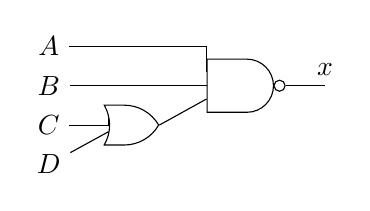
\begin{tikzpicture}[label distance=1mm]
            \node (A) at (0,1.5) {$ A $};
            \node (B) at (0,1) {$ B $};
            \node (C) at (0,0.5) {$ C $};
            \node (D) at (0,0) {$ D $};
            \node[or gate US, draw, logic gate inputs=nn] at ($(D)+(1,0.5)$) (Or0) {};
            \node[nand gate US, draw, logic gate inputs=nnn] at ($(Or0.output)+(1,0.5)$) (Nand0) {};
            \draw (C) -| (Or0.input 1);
            \draw (D) -- (Or0.input 2);
            \draw (A) -| (Nand0.input 1);
            \draw (B) -| (Nand0.input 2);
            \draw (Or0.output) -- (Nand0.input 3);
            \draw (Nand0.output) -- ([xshift=0.5cm]Nand0.output) node[above] {$ x $};
        \end{tikzpicture}\\\\
  \\\\      
b) 	
		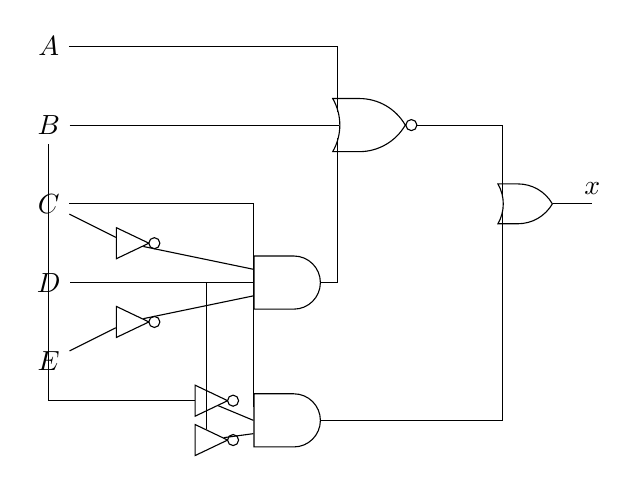
\begin{tikzpicture}[label distance=2mm]
			\node (A) at (0,4) {$ A $};
            \node (B) at (0,3) {$ B $};
            \node (C) at (0,2) {$ C $};
            \node (D) at (0,1) {$ D $};
            \node (E) at (0,0) {$ E $};
            \node[nor gate US, draw, logic gate inputs=nnn] at ($(B)+(4,0)$) (Nor0) {};
            \node[and gate US, draw, logic gate inputs=nnn] at ($(D)+(3,0)$) (And0) {};
            \node[and gate US, draw, logic gate inputs=nnn] at ($(E)+(3,-0.75)$) (And1) {};
            \node[or gate US, draw, logic gate inputs=nn] at ($(C)+(6,0)$) (Or0) {};
            \node[not gate US, draw, logic gate inputs=n] at ($(C)+(1,-0.5)$) (Not0) {};
            \node[not gate US, draw, logic gate inputs=n] at ($(E)+(1,0.5)$) (Not1) {};
            \node[not gate US, draw, logic gate inputs=n] at ($(E)+(2,-0.5)$) (Not2) {};
			\node[not gate US, draw, logic gate inputs=n] at ($(E)+(2,-1)$) (Not3) {};
			\draw (A) -| (Nor0.input 1);
			\draw (B) -- (Nor0.input 2);
			\draw (B) |- (Not2);
			\draw (C) -- (Not0);
			\draw (D) -- (And0.input 2);
			\draw (E) -- (Not1);
			\draw (D) -| (Not3);
			\draw (Not0) -- (And0.input 1);
			\draw (Not1) -- (And0.input 3);
			\draw (And0.output) -| (Nor0.input 3);
			\draw (C) -| (And1.input 1);
			\draw (Not2) -- (And1.input 2);
			\draw (Not3) -- (And1.input 3);
			\draw (Nor0.output) -| (Or0.input 1);
			\draw (And1.output) -| (Or0.input 2);			\draw (Or0.output) -- ([xshift=0.5cm]Or0.output) node[above] {$ x $};
			
        \end{tikzpicture}\\\\
c)
        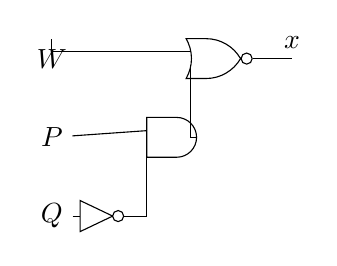
\begin{tikzpicture}[label distance=1mm]
            \node (W) at (0,2) {$ W $};
            \node (P) at (0,1) {$ P $};
            \node (Q) at (0,0) {$ Q $};
            \node[nor gate US, draw, logic gate inputs=nn] at ($(W)+(2,0)$) (Nor0) {};
            \node[and gate US, draw, logic gate inputs=nn] at ($(P)+(1.5,0)$) (And0) {};
            \node[not gate US, draw, logic gate inputs=n] at ($(Q)+(0.5,0)$) (Not0) {};
            \draw (W) |- (Nor0.input 1);
            \draw (P) -- (And0.input 1);
            \draw (Q) -- (Not0);
            \draw (Not0) -| (And0.input 2);
            \draw (And0.output) -| (Nor0.input 2);
            \draw (Nor0.output) -- ([xshift=0.5cm]Nor0.output) node[above] {$ x $};
        \end{tikzpicture}\\\\
  \\\\ 
d)
        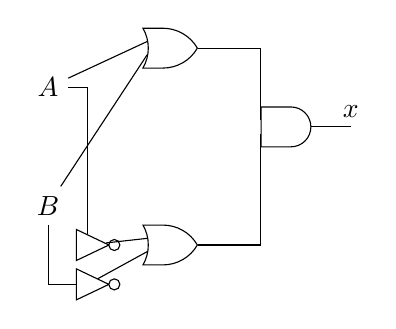
\begin{tikzpicture}[label distance=1mm]
            \node (A) at (0,1) {$ A $};
            \node (B) at (0,-0.5) {$ B $};
            \node[or gate US, draw, logic gate inputs=nn] at ($(A)+(1.5,0.5)$) (Or0) {};
            \node[or gate US, draw, logic gate inputs=nn] at ($(B)+(1.5,-0.5)$) (Or1) {};
            \node[and gate US, draw, logic gate inputs=nn] at ($(A)+(3,-0.5)$) (And0) {};
            \node[not gate US, draw, logic gate inputs=n] at ($(B)+(0.5,-0.5)$) (Not0) {};
            \node[not gate US, draw, logic gate inputs=n] at ($(B)+(0.5,-1)$) (Not1) {};
            \draw (A) -- (Or0.input 1);
            \draw (B) -- (Or0.input 2);
            \draw (A) -| (Not0);
            \draw (B) |- (Not1);
            \draw (Not0) -- (Or1.input 1);
            \draw (Not1) -- (Or1.input 2);
            \draw (Or0.output) -| (And0.input 1);
            \draw (Or1.output) -| (And0.input 2);
            \draw (And0.output) -- ([xshift=0.5cm]And0.output) node[above] {$ x $};
        \end{tikzpicture}\\\\
  \\\\ 
\problem{}{0}
\solution
\textcolor{blue}
Truth table:\\
  \begin{center}
            \begin{tabular}{|c|c|c||c|}
                \hline
                M&N&Q&R  \\
                \hline
                0&0&0&0  \\
                \hline
                0&0&1&0  \\
                \hline
                0&1&0&0  \\
                \hline
                1&0&0&0  \\
				\hline
                0&1&1&1  \\                
                \hline
                1&0&1&1  \\
                \hline
                1&1&0&0  \\
                \hline
                1&1&1&1  \\
                \hline
            \end{tabular}
        \end{center}
To find the sum-of-products expression we should find DNF: 
\begin{equation}
	(\overline{M} \cdot N \cdot Q) + (M \cdot \overline{N} \cdot Q) + (M \cdot N \cdot Q)
\end{equation}

We see common factor Q, and using Distributive rule, we can take it out:
\begin{equation}
	Q \cdot (\overline{M} \cdot N + M \cdot \overline{N}+ M \cdot N )
\end{equation}
Now let's use it once more inside of bracket:
\begin{equation}
	Q \cdot (\overline{M} \cdot N + M \cdot (\overline{N}+ N ))
\end{equation}
Now using compliment law, we get rid of second N in bracket. 
\begin{equation}
	Q \cdot (\overline{M} \cdot N + M )
\end{equation}
Again using distributive equation:
\begin{equation}
	Q \cdot ((\overline{M} + M )\cdot(M + N) )
\end{equation}
Again, complement, and $1*w =w$ formula brings us to
\begin{equation}
	Q \cdot (N + M )
\end{equation}
Check the truth table, and they correspond, so the answer is correct.
\\\\
\problem{}{0}
\solution
\textcolor{blue}
a) First, left part:
\begin{equation}
	X + (\overline{X} \cdot Y )
\end{equation}
\begin{center}
            \begin{tabular}{|c|c||c|}
                \hline
                X&Y&Q \\
                \hline
                0&0&0 \\
                \hline
                0&1&1 \\
                \hline
                1&0&1 \\
                \hline
                1&1&1 \\
                \hline
            \end{tabular}
        \end{center}
Now, right part:
\begin{equation}
	X + Y 
	\end{equation}
\begin{center}
            \begin{tabular}{|c|c||c|}
                \hline
                X&Y&Q \\
                \hline
                0&0&0 \\
                \hline
                0&1&1 \\
                \hline
                1&0&1 \\
                \hline
                1&1&1 \\
                \hline
            \end{tabular}
\end{center}
We can see, that they are same.
\\\\
b) First, left part:
\begin{equation}
	\overline{X} + (X \cdot Y )
\end{equation}
\begin{center}
            \begin{tabular}{|c|c||c|}
                \hline
                X&Y&Q \\
                \hline
                0&0&1 \\
                \hline
                0&1&1 \\
                \hline
                1&0&0 \\
                \hline
                1&1&1 \\
                \hline
            \end{tabular}
        \end{center}
Now, right part:

\begin{equation}
	\overline{X} + Y 
	\end{equation}
\begin{center}
            \begin{tabular}{|c|c||c|}
                \hline
                X&Y&Q \\
                \hline
                0&0&1 \\
                \hline
                0&1&1 \\
                \hline
                1&0&0 \\
                \hline
                1&1&1 \\
                \hline
            \end{tabular}
\end{center}
        

\problem{}{0}
\solution
\textcolor{blue}
a) \begin{equation}
	A + 1 = 1
	\end{equation}\\
b) \begin{equation}
	A \cdot A = A
	\end{equation}\\
c)  \begin{equation}
	B \cdot \overline{B} = 0
	\end{equation}\\
d) \begin{equation}
C + C = C
	\end{equation}\\
e) \begin{equation}
	x \cdot 0 = 0 
	\end{equation}\\
f)\begin{equation}
	D \cdot 1 = D 
	\end{equation}\\
g)\begin{equation}
	D + 0 = D 
	\end{equation}\\
h)\begin{equation}
	C + \overline{C} = 1 
	\end{equation}\\
i)\begin{equation}
	G + G\cdot F = G \cdot (1+F) = G
	\end{equation}\\
j) \begin{equation}
	y + \overline{w}\cdot y  = y \cdot (1 + \overline{w}) = y
	\end{equation}\\
   
\problem{}{0}
\solution
DeMorgan's Theorem:
   \begin{equation}
	\overline{(A+B)} = \overline{A} \cdot \overline{B}
	\end{equation}\\
Proof: 
 First, left part:
\begin{equation}
\overline{(A+B)}
\end{equation}
\begin{center}
            \begin{tabular}{|c|c||c|}
                \hline
                A&B&R \\
                \hline
                0&0&1 \\
                \hline
                0&1&0 \\
                \hline
                1&0&0 \\
                \hline
                1&1&0 \\
                \hline
            \end{tabular}
        \end{center}
Now, right part:

\begin{equation}
	\overline{A} \cdot \overline{B}
	\end{equation}
\begin{center}
            \begin{tabular}{|c|c||c|}
                \hline
                A&B&Q \\
                \hline
                0&0&1 \\
                \hline
                0&1&0 \\
                \hline
                1&0&0 \\
                \hline
                1&1&0 \\
                \hline
            \end{tabular}
\end{center}    
        
Next theorem:
\begin{equation}
	\overline{(A\cdot B)} = \overline{A} + \overline{B}
	\end{equation}\\
Proof: 
 First, left part:
\begin{equation}
\overline{(A\cdot B)}
\end{equation}
\begin{center}
            \begin{tabular}{|c|c||c|}
                \hline
                A&B&R \\
                \hline
                0&0&1 \\
                \hline
                0&1&1 \\
                \hline
                1&0&1 \\
                \hline
                1&1&0 \\
                \hline
            \end{tabular}
        \end{center}
Now, right part:

\begin{equation}
	\overline{A} + \overline{B}
	\end{equation}
\begin{center}
            \begin{tabular}{|c|c||c|}
                \hline
                A&B&Q \\
                \hline
                0&0&1 \\
                \hline
                0&1&1 \\
                \hline
                1&0&1 \\
                \hline
                1&1&0 \\
                \hline
            \end{tabular}
\end{center}    
      
\problem{}{0}
\solution 
 The sum of products expression is 
 \begin{equation}
	\overline{A} \cdot \overline{B} \cdot \overline{C} \cdot D + \overline{A} \cdot \overline{B} \cdot C \cdot D + \overline{A} \cdot B \cdot \overline{C} \cdot D + \overline{A} \cdot B \cdot C \cdot D + A \cdot \overline{B} \cdot \overline{C} \cdot \overline{D} + A \cdot B \cdot \overline{C} \cdot D + A \cdot B \cdot C \cdot D 
	\end{equation}
Simplify: 
Applying associative and distributive rules:
 \begin{equation}
	\overline{A} \cdot (\overline{B} \cdot \overline{C} \cdot D + \overline{B} \cdot C \cdot D + B \cdot \overline{C} \cdot D + B \cdot C \cdot D)  + A \cdot (\overline{B} \cdot \overline{C} \cdot \overline{D} + B \cdot \overline{C} \cdot D + B \cdot C \cdot D )
	\end{equation}
Distributive rule:
\begin{equation}
	\overline{A} \cdot (\overline{B} \cdot (\overline{C} \cdot D + C \cdot D ) + B \cdot (\overline{C} \cdot D + C \cdot D))  + A \cdot (\overline{B} \cdot \overline{C} \cdot \overline{D} + B \cdot (\overline{C} \cdot D + C \cdot D))
	\end{equation}
Distributive rule:
\begin{equation}
	\overline{A} \cdot ((\overline{B} + B)\cdot (\overline{C} \cdot D + C \cdot D ))  + A \cdot (\overline{B} \cdot \overline{C} \cdot \overline{D} + B \cdot (D \cdot (\overline{C}+ C )))
	\end{equation}
Complement rule:
\begin{equation}
	\overline{A} \cdot ((1)\cdot (\overline{C} \cdot D + C \cdot D ))  + A \cdot (\overline{B} \cdot \overline{C} \cdot \overline{D} + B \cdot (D \cdot (1 )))
	\end{equation}
De Morgan law and distributive rule:
\begin{equation}
	\overline{A} \cdot ((\overline{C}  + C ) \cdot D )  + A \cdot (\overline{B} \cdot \overline{C} \cdot \overline{D} + B \cdot D )
	\end{equation}
Complement rule and de Morgan law:
\begin{equation}
	\overline{A} \cdot D + A \cdot (\overline{B} \cdot \overline{C} \cdot \overline{D} + B \cdot D )
	\end{equation}
Since, they have identical truth tables, we did no mistake and found the simplified version of equation.
 
\problem{}{0}
\solution
First we generate the table for 4 variables. We fill it with combinations from sums of products.
\begin{center}
            \begin{tabular}{|c|c|c|c|c|}
                \hline
                &$\overline{C} \cdot \overline{D}$&$\overline{C}\cdot D$&$C\cdot D$&$C\cdot \overline{D}$ \\ \hline
                $\overline{A}\cdot \overline{B}$&0&1&1&0 \\ \hline
                $\overline{A}\cdot B$&0&1&1&0 \\ \hline
                $A\cdot B$&0&1&1&0 \\ \hline
                $A\cdot\overline{B}$&1&0&0&0 \\ \hline
            \end{tabular}
        \end{center} 
We can see one isolated case: $A\cdot \overline{B}\cdot \overline{C} \cdot \overline{D}$
Now, we have to loop through other groups and eliminate bad options.
Then, second we loop through groups of 4. There are 2 of them. One containing squares 2,3,6,7 and the other one containing 6,7,10,11. That give us next two elements: $\overline{A} \cdot D$ and $B \cdot D$. Therefore the final equation is $A\cdot \overline{B}\cdot \overline{C} \cdot \overline{D} + \overline{A} \cdot D + B \cdot D$
        
        
\end{document}